\begin{frame}{Text and Image in Beamer}
    \begin{columns}
    \column{0.4\textwidth}
        \begin{enumerate}
            \item This is a list
            \item This has a sub-list
                \begin{itemize}
                    \item This is a sub-list
                    \item This has bullet points
                \end{itemize}
            \item The list has numbers    
        \end{enumerate}
    \column{0.6\textwidth}
        \begin{figure}
        \centering
        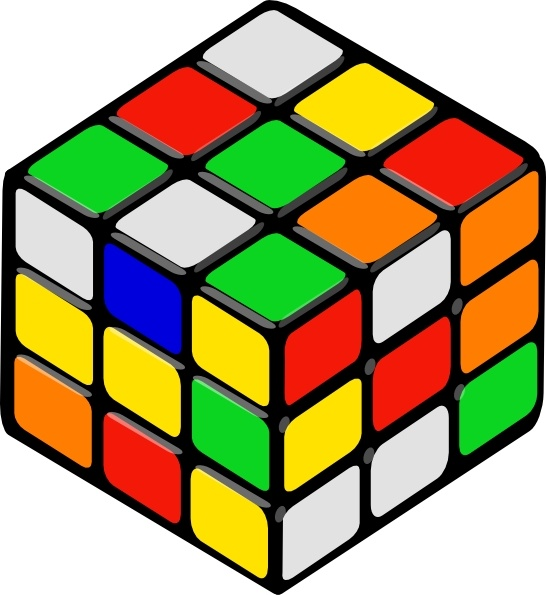
\includegraphics[scale=0.2]{images/illustrate/illus1.jpg}
        \caption{Random Image}
        \end{figure}
    \end{columns}
\end{frame}

\begin{frame}{same}
    \begin{enumerate}
            \item This is a list
            \item This has a sub-list
                \begin{itemize}
                    \item This is a sub-list
                    \item This has bullet points
                \end{itemize}
            \item The list has numbers
            \item This is a list
            \item This has a sub-list
                \begin{itemize}
                    \item This is a sub-list
                    \item This has bullet points
                \end{itemize}
            \item The list has numbers   
            \item This is a list
            \item This has a sub-list
                \begin{itemize}
                    \item This is a sub-list
                    \item This has bullet points
                \end{itemize}
            \item The list has numbers   
            \item This is a list
            \item This has a sub-list
          
            \item The list has numbers   
        \end{enumerate}
\end{frame}